\documentclass{book}
\usepackage{amsmath,amsfonts,	%packages for formatting math
	amsthm,						%theorem environment
	gensymb, 					%generic math symbols (e.g., degree)
	commath} 					%math formatting for diff eq
\usepackage[dvips, pdftex]{graphicx}		%graphics handling
\usepackage{amssymb, 	%math symbols
	mathrsfs} 			%uppercase script in math mode

\usepackage{booktabs} %nice tables

\usepackage[T1]{fontenc} % for copy/paste
\usepackage{lmodern}

\usepackage{units} %easily typeset units
\usepackage{fancyhdr} %more/better control of header/footer
\usepackage{float} %control float placement

\usepackage{caption, subcaption} %multiple floats with indiv. caption

\usepackage{multirow} %allow cells in tables to span multiple rows

%define a bunch of colors to be used NOTE: some of these are used only in personal style files and should be moved there
\usepackage{xcolor, colortbl}
\definecolor{maroon}{rgb}{0.69,0.18,0.38}
\definecolor{goldenrod}{rgb}{0.85, 0.65, 0.13}
\definecolor{ltgray}{rgb}{0.75, 0.75, 0.75}
\definecolor{gray}{rgb}{0.5, 0.5, 0.5}
\definecolor{ltyellow}{rgb}{1, 1, 0.6}
\definecolor{turq}{rgb}{.11, .55, 0.55}
\definecolor{dkgreen}{rgb}{0.13, 0.55, 0.13}

\usepackage{bytefield} %for pretty byte representation
\newlength{\maxheight} %set up some new commands to be used in bytefield
\setlength{\maxheight}{\heightof{W}}

\newcommand{\baselinealign}[1]{%
\centering
\raisebox{0pt}[\maxheight][0pt]{#1}%
}


%define a command to be used we notating we have "other" code in the source not shown
\newcommand{\codefill}{\centering$\longrightarrow$\hfill{\color{gray}\rule[0.1\baselineskip]{0.5\linewidth}{2pt}}\hfill$\longleftarrow$}

\usepackage[compact]{titlesec} %reduce the spacing around section/subsection/etc titles

\usepackage{upquote} %make quotes single

\usepackage{fancyvrb} %fancy verbatim

\usepackage{tikz, atbegshi} %these are used for highlighting

% change this to customize the appearance of the highlight
\tikzstyle{highlighter} = [
  ltyellow,
  line width = \baselineskip,
]

% enable these two lines for a more human-looking highlight
%\usetikzlibrary{decorations.pathmorphing}
%\tikzstyle{highlighter} += [decorate, decoration = random steps]

% implementation of the core highlighting logic; do not change!
\newcounter{highlight}[page]
\newcommand{\tikzhighlightanchor}[1]{\ensuremath{\vcenter{\hbox{\tikz[remember picture, overlay]{\coordinate (#1 highlight \arabic{highlight});}}}}}
\newcommand{\bh}[0]{\stepcounter{highlight}\tikzhighlightanchor{begin}}
\newcommand{\eh}[0]{\tikzhighlightanchor{end}}
\AtBeginShipout{\AtBeginShipoutUpperLeft{\ifthenelse{\value{highlight} > 0}{\tikz[remember picture, overlay]{\foreach \stroke in {1,...,\arabic{highlight}} \draw[highlighter] (begin highlight \stroke) -- (end highlight \stroke);}}{}}}
%--------------------------


\usepackage{bookmark} %allow bookmarks (Table of Contents in PDF)

\VerbatimFootnotes %make sure verbatim environments can exist in bookmarks
\DefineVerbatimEnvironment{code}{Verbatim}{fontsize=\small}

%define an "aside" environment
\newtheoremstyle{aside_style}{10pt}{5pt}{\itshape}{}{\bfseries}{:}{\newline}{}
\theoremstyle{aside_style}
\newtheorem*{myaside}{Aside}
\newenvironment{aside}
	{\par\noindent\hrulefill\begin{myaside}}
	{\par\noindent\hrulefill\end{myaside}}

\usepackage{listings}%for "pretty code" input

%get some style files for different types of listings:
\usepackage{idl_listing_def} %personal styling for IDL syntax
%\usepackage{latex_code_listing} %define an environment for LaTex code (personal)
%\usepackage{bash_code_listing} %and one for bash (personal)

\usepackage{typedref} %to use \sectionref, etc.

\refname{problem}{Problem}{Problems} %define a problem class to reference Problems
\refname{equation}{Equation}{Equations} %define an equationref to print equation (x.x)

\usepackage{makeidx} %provide an index
\makeindex

%define our header/footer
\pagestyle{fancy}
\fancyfoot{} %clear the footer
\fancyfoot[OR, EL]{\thepage}
\fancyfoot[ER, OL]{\tiny{Last edited: \today}}

\renewcommand{\familydefault}{\sfdefault} %use sanserif font for the document
\usepackage{sfmath} %math roman font the default for math

%define margins for the document
\newcommand{\thispagewidth}{6.75in}

\setlength{\topmargin}{0pt} \setlength{\topskip}{0pt}
\setlength{\headheight}{12pt} \setlength{\headsep}{10pt}
\setlength{\headwidth}{\thispagewidth}
\setlength{\textheight}{9in}\setlength{\textwidth}{\thispagewidth}
\setlength{\footskip}{15pt}
\setlength{\hoffset}{0in}\setlength{\voffset}{0in}

\setlength{\marginparwidth}{0.6in}

\setlength{\oddsidemargin}{-.15in} 
\setlength{\evensidemargin}{-.15in} 
\setlength{\parindent}{0in}
\setlength{\parskip}{20pt} 
\renewcommand{\headrulewidth}{1pt}

%provide a variable to note if we're generating notes for class or instructor
\newif\ifshownotes
\shownotestrue
\shownotesfalse

\ifshownotes %if we're compiling for the instructor, provide a visual output
  \usepackage{background}
  \backgroundsetup{%
	  scale=3,       %% change accordingly
	  angle=0,       %% change accordingly
	  opacity=.6,    %% change accordingly
	  color =black,  %% change accordingly
	  position={1in, 0.25in},
	  contents={CLASS NOTES}
	}
\fi

%uncomment the following to show labels for tables, figures, etc.
%\usepackage[]{showlabels} %make reference labels, but redefine the font/color
%\renewcommand{\showlabelfont}{\small}
%\renewcommand{\showlabelsetlabel}[1]{\colorbox{red}{\showlabelfont #1}}

\newcommand{\classnote}[1]{\ifshownotes \marginpar[\color{gray} #1]{\color{gray} #1} \fi} %make a note in the margin

\newcommand{\todo}[1]{{\color{blue}{\rule{0.5in}{1in}} Todo: #1}} %add a blue box for space, and add inline note to do something

\newcommand{\link}[1]{\href{#1}{\nolinkurl{#1}}} %web site links

%\write18{./findtodo.sh} %shell escape must be enabled for this to work

\begin{document}

\setcounter{chapter}{16} %assume 11 chapters have already been done
\chapter{IDL, FTP, and MODIS}

In this section, we'll take a look at how to retrieve MODIS files from a file transfer protocal (FTP) site and 
write a routine to pull these images from the server based on certain criteria defined by the user. 

%***********************************            Section 1           *******************************************************
\section{Introduction}
Popular sites for downloading NASA satellite imagery are the USGS Earth Explorer and the USGS Global Visualization Viewer (GLOVIS).
These websites have interactive maps and all sorts of features and options. However, going through the motions of navigating the map,
picking out options, and requesting your download for each image you need can be tedious at best if your analysis requires more than a few
images.

FTP servers are quick and powerful tools for downloading data and, with a little background knowledge,
we can develop tools for automating the process based on the user's needs. In this tutorial, we'll review string operations, 
initialize an IDLnetURL object, set the object's properties, and call its methods in order to communicate with the server. 
This tutorial is constructed to enable the batch downloading of MOD09A1 and MYD09A1 products. 
The methodology of the following sections can be applied to several other MODIS products, 
but because there are literally hundreds of products, the syntax and structure of these procedures may require some extra tweaking.


But first, a little background information on MODIS.



\begin{aside}
We've used objects before, starting in Chapter 5 when we added various elements to a list using the "Add" method. 
We also created a cgMap object in Chapter 10 to make mapping easier.
\end{aside}





\pagebreak

%***********************************            Section 2           *******************************************************
\section{What's in a name? MODIS naming conventions}\label{MODISname}

The Moderate Resolution Imaging Spectroradiometer (MODIS) instrument is a NASA Earth Observation on two different satellites, Aqua and Terra.
Imagery captured is downlinked and sent to the Land Processes Distributed Active Archive Center (LPDAAC) where raw, level 1 data is processed 
into higher level products. 

As with all publicly available NASA data sets, imagery from the MODIS sensors follow a very specific naming convention. This helps with
organization and allows the user to quickly determing the product, date, and location of the file in question. Let's look at an example of a 
file and break it down from left to right:

\begin{lstlisting}
                 MOD09A1.A2008193.h00v08.005.2008019201033.hdf
\end{lstlisting}
\vskip-20pt
MOD09A1 is a classic Level-3 reflectance product. It's worth noting that the second letter of the product name indicates the satellite(s) that this
image was taken from. In this case, MOD indicates that this image was taken on the Terra satellite. MYD products came from Aqua, and MCD products
are combined products made from imagery from both Aqua and Terra. Some products are satellite-specific, while others are not. Believe it
or not, the file beginning with

\begin{lstlisting}
                 MYD09A1.A2008193.h00v08.005
\end{lstlisting}
\vskip-20pt
is an actual product from Aqua that you can download just like our original from Terra! This coincidence might prove useful to us later...

Each section of our filename is separated by periods. After our product name comes the year and date in the Julian calendar. For this file, we're looking
at an image taken on (193, 2008) or July 11, 2008. \footnote{Be sure to account for leap years!}

Next, we have our horizontal and vertical grid indices. MODIS images are arranged in tiles roughly 10x10 degrees. It's important to note that these
parameters are zero-padded to the left in the file name.

\begin{figure}[H]
\centering
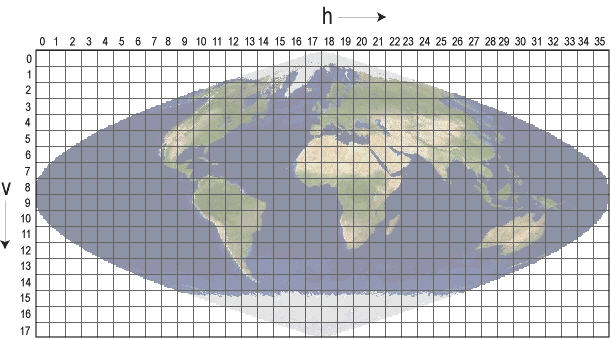
\includegraphics[width=0.75\textwidth]{images/modis_sinusoidal_grid}
\caption{The MODIS sinusioidal grid projection}
\label{modgrid}
\end{figure}

\pagebreak
Next, we have 005, which indicates that this product is located within MODIS collection \#5. This collection contains all of the products
we might need, so we'll keep this at 5 for the purposes of this tutorial. 

The next section is the processing date, which is a bit of a wildcard. You may have noticed that, up until now, each of our parameters in this
file name are easy to control and predict while we're "shopping" for MODIS images. Collecting this information will be an important step 
in our process of automating our downloads.

Lastly, we have the file extension .hdf. This is a common and well-documented file type for satellite imagery. We can even pop it open in our 
netcdf viewer. Nice!

%***********************************            Section 3           *******************************************************
\section{Any way you want it: Predicting MODIS filenames}

The key to this method of downloading images is the consistency of the MODIS file naming convention. 
By parameterizing each element of the filename, we can build "partial" filenames that can be used to search for the image later.
In essence, we can use user input to "build" this:

\begin{lstlisting}
                 MOD09A1.A2008193.h00v08.005
\end{lstlisting}

in order to search for and download this file:

\begin{lstlisting}
                 MOD09A1.A2008193.h00v08.005.2008019201033.hdf
\end{lstlisting}

As you can probably imagine, this will require many string operations.
We'll write a procedure with a helper function or two to make this happen. Let's get started.

\begin{idl}
%{\codefill}% 
%\bh%;file documentation%\eh%
%\bh%PRO ess_download_modis%\eh%
%\bh%;routine documentation%\eh%

%\bh%compile_opt idl2%\eh%

%\bh%;error catcher:%\eh%
%\bh%CATCH, theError%\eh%
%\bh%IF theError NE 0 THEN BEGIN%\eh%
%\bh%  CATCH, /cancel%\eh%
%\bh%  HELP, /LAST_MESSAGE, OUTPUT=errMsg%\eh%
%\bh%  FOR i=0, N_ELEMENTS(errMsg)-1 DO print, errMsg[i]%\eh%
%\bh%  RETURN%\eh%
%\bh%ENDIF%\eh%

%\bh%;format input parameters as strings and zero-fill%\eh%

%\bh%;build the partial filename%\eh%

%\bh%;build url path from filename parameters%\eh%

%\bh%;instantiate a new IDLnetURL object and connect to the server%\eh%

%\bh%;return a directory listing from the current ftp path%\eh%

%\bh%;search for and store "long" file name of desired image%\eh%

%\bh%;change directories to the desired file%\eh%

%\bh%;"get" the file%\eh%

%\bh%;object cleanup%\eh%

%\bh%END%\eh%
%{\codefill}% 
\end{idl}

Let's see what we've got cooking here in the comments. First, we start formatting our parameters as strings, and then we'll do whatever "zero-fill" means,
so we should probably set up some input parameters. Keeping things in order from the naming convention,
we'll set the product\footnote{Remember that "Product" is a reserved word in IDL}
, year, Julian day, horizontal, and vertical grid indices:

\begin{idl}
PRO ess_download_modis%\bh%, imgProd, imgYear, imgDate, imgHgrid, imgVgrid%\eh%
\end{idl}

Now we have access to all of the parameters of our filename as passed to us by the user. What format will all of these inputs be in? 
Our product name will be forced to come in as a string, but the next four inputs will probably be long integers by default. 
Since we need everything to be formatted as a string, we'll make sure our product is in all caps and set up our year variable:

\begin{idl}
;format all input parameters as strings, zero-filling as necessary
%\bh%prod = STRUPCASE(imgProd)%\eh%
%\bh%year = STRING(imgYear)%\eh%
\end{idl}

Our next parameters aren't quite so simple. Remember that the grid indices are zero-padded to the left? (h00v05)
It turns out our Julian date parameter is also zero-padded to three places\footnote{e.g. an image on January 9 gives us MOD09A1.A2008009.h20v02.005.2008020034715}
We'll need to find a way to format our inputs so that our long integers become strings that fill precisely two or three spaces, filling in zeros as needed.
Let's write a quick helper function
\footnote{While we're writing this as a helper function for this procedure, note that there's nothing MODIS-specific that we'll be doing with this function.
It may be worth it to save this function as its own file to be used in other settings as well.}
 to handle this:

\begin{idl}
%{\codefill}% 
%\bh%FUNCTION ess_download_modis_zerofill, strIn, fill%\eh%
%\bh%;function documentation%\eh%
  
%\bh%compile_opt idl2%\eh%

%\bh%;format strIn by converting to a string and removing all leading spaces %\eh%
    
%\bh%;determine the number of leading zeros needed%\eh%
    
%\bh%;conditionally add leading zeros to the parameter%\eh%
  
%\bh%;return the result%\eh%

%\bh%END%\eh%

PRO ess_download_modis, imgProd, imgYear, imgDate, imgHgrid, imgVgrid
%{\codefill}% 
\end{idl}

Here we have a function with two inputs, the string we need to format, and the fill number.
As it turns out, the STRING() typecasting function adds some annoying spaces at the beginning of your output. Let's use STRTRIM to remove them:

\begin{idl}
;format strIn by converting to a string and removing all leading spaces
%\bh%strIn = STRTRIM( STRING(strIn),1 )%\eh%
\end{idl}

Next, let's compare how long this formatted string is with how many spaces the caller wants filled:

\begin{idl}
;determine the number of leading zeros needed
%\bh%zf = fill - STRLEN(strIn)%\eh%
\end{idl}

Now let's think about how to conditionally add zeros to our string based on this fill.
A couple of IF's should do the trick: zf should tell us how many zeros to concatenate.
If zf is zero, that means our string is good to go, so we'll leave it alone and return it.

\begin{idl}
;conditionally add leading zeros to the parameter
%\bh%IF zf EQ 2 THEN zFill = '00' + strIn $%\eh%
%\bh%  ELSE IF zf EQ 1 THEN zFILL = '0' + strIn $%\eh% 
%\bh%  ELSE zFill = strIn%\eh%  

;return the result
%\bh%RETURN, zFill%\eh%

END
\end{idl}

Excellent. Now back to our procedure, let's format the date and grid indices using our new helper function:
Let's add a temporary print statement to make sure we got it right, too:

\begin{idl}
;format all input parameters as strings, zero-filling as necessary
prod = STRUPCASE(imgProd)
year = STRING(imgYear)
%\bh%date = ess_download_modis_zerofill(imgDate, 3)%\eh%
%\bh%hInd = ess_download_modis_zerofill(imgHgrid, 2)%\eh%
%\bh%vInd = ess_download_modis_zerofill(imgVgrid, 2)%\eh%
%\bh%print, prod, year, date, hInd, vInd%\eh%


IDL> ess_download_modis, 'MOD09A1', 2001, 49, 10,5
\end{idl}

Formatting is a little funky, but it sure looks like we got it right. Now let's put all of these strings together. At first glance, it may seem like a simple concatenation operation between our variables and a bunch of dots.
However, because of the way typecasting works, sometimes we end up with extra spaces in places we don't want. Here, if we run:

\begin{idl}
print, prod + '.A' + year + date + '.h' + hInd + 'v' + vInd
\end{idl}

IDL would return MOD09A1.A \ \ \   2001049.h10v05. Not what we wanted. Let's try a combination of STRSPLIT and STRJOIN.
STRSPLIT will cut through any excess whitespace in a string and return each element as an independent string with the /EXTRACT keyword.
STRJOIN will the re-concatenate these for us, much like the + operator:

\begin{idl}
;build the partial filename
%\bh%partialFname = STRJOIN(STRSPLIT(prod + '.A' + year + date + '.h' $%\eh%
%\bh%  + hInd + 'v' + vInd, /EXTRACT) )%\eh%
\end{idl}

Run a quick print statement to check your output.
With the same parameters, you should end up with something like MOD09A1.A2001049.h10v05.
Now that we have a partial filename, let's get connected and search for our images!


%***********************************            Section 4           *******************************************************
\section{Communicating with the outside: IDLnetURL}

Our primary tool for downloading these images will be the IDLnetURL package.
Documentation for these objects can be found here \link{http://www.exelisvis.com/docs/IDLnetURL.html}
In order to connect and download the files we need, we'll instantiate an IDLnetURL object, set its parameters, 
and then call the various methods included in the object to interact with the server. 

The FTP server we'll be using is \link{ftp://ladsftp.nascom.nasa.gov} Feel free to navigate there in a browser and explore.
The data we need are located in the directory \textbackslash allData\textbackslash 5.
It is important to get familiar with the directory structure. The data are sorted into product name, year, and Julian date directories.
After that, we'll have to sort through a page of file names sorted by their grid indices to pick out the images we want.
For testing, pick out a MOD09A1 file and use its parameters. This way, you can guarantee that the image exists when you start talking to the server.

Now, let's set up some of our connection parameters. 
For the host, we'll leave out the beginning "ftp://" because we have a property that we can set to tell the object that we're using an FTP instead of a URL.
To set the path, we'll dance the same jig we did building the partial filename, this time leaving out the grid indices.

\begin{idl}
;build url path from filename parameters
%\bh%urlHost = 'ladsftp.nascom.nasa.gov'%\eh%
%\bh%urlPath = STRJOIN(STRSPLIT('allData/5/' + prod + '/' $%\eh%
%\bh%  + year + '/' + date + '/', /EXTRACT) )%\eh%
\end{idl}

Now, we have everything we need to instantiate our IDLnetURL object.
The OBJ\_NEW() function creates a new object and allows you to set properties, much like keywords for a procedure.
There are built-in methods to set each property one-by-one, but this tends to be tedious for more that a few properties.
Let's set them all at once and then discuss:

\begin{idl}
%{\codefill}% 
;instantiate a new IDLnetURL object and connect to the server
%\bh%oUrl = OBJ_NEW('IDLnetUrl', $%\eh%
%\bh%                URL_SCHEME='ftp', $%\eh%
%\bh%                FTP_CONNECTION_MODE=0, $%\eh%
%\bh%                URL_HOST=urlHost, $%\eh%
%\bh%                URL_Port=21, $%\eh%
%\bh%                URL_USERNAME='anonymous', $%\eh%
%\bh%                URL_PASSWORD='', $%\eh%
%\bh%                URL_PATH=urlPath)%\eh%
%{\codefill}% 
\end{idl}

There's a lot going on here, so let's break it down. We've created a new variable, oUrl, to be our object. 
The first property of our function sets the object type: here, we need an 'IDLnetURL' object.
Next, we set the URL\_SCHEME property to 'ftp.'
CONNECTION\_MODE gets set to 0 which, per the documentation, establishes a passive connection.
Certain servers require a passive connection and ladsftp is one of them.
We've already prepared our URL\_HOST property, so we just plug it in here.

The default Transmission Connection Port (TCP) for sending and receiving files from an FTP server is 21, so we'll set it here just in case.
All ftp servers require a login, but ladsftp, like many other servers, is an "Anonymous" server.
This means that a secure username and password are not required for accessing files for downloading.
Instead, your browser automatically logs you in as username \textit{anonymous} with a null character password whenever you browse there.
For IDLnetURL, the process is not automated, so we'll supply the appropriate "credentials" ourselves.

Lastly, we'll plug in the URL path that we've already created.
You may also want to add the property VERBOSE=1 in order to see any responses from the server as you poke around on the server.

This all may sound well and good, but does it actually work? In order to test, let's create a little main level program with some hard-coded values.
This should do the trick:

\begin{idl}
%{\codefill}%
END

%\bh%url = 'allData/5/MOD09A1/2001/049/MOD09A1.A2001049.h10v05.005.2006362053450.hdf'%\eh%
%\bh%host = 'ladsftp.nascom.nasa.gov'%\eh%

%\bh%oUrl = OBJ_NEW('IDLnetUrl', $%\eh%
                %\bh%URL_SCHEME='ftp', $%\eh%
               %\bh% FTP_CONNECTION_MODE=0, $%\eh%
                %\bh%URL_HOST=host, $%\eh%
                %\bh%URL_Port=21, $%\eh%
                %\bh%URL_USERNAME='anonymous', $%\eh%
                %\bh%URL_PASSWORD='', $%\eh%
                %\bh%URL_PATH=url)%\eh%
   
%\bh%void = oURL->Get(FILENAME='test.hdf')%\eh%

%\bh%OBJ_DESTROY, oURL%\eh%

%\bh%END ; main level program%\eh%
%{\codefill}%
\end{idl}

Now, a couple of things to note here. 
Most striking should be this new OBJ\_DESTROY command.
This step is crucial because we need to close all of our connections and get rid of any new objects we create. 
It may not seem necessary for a simple routine like this, but in larger projects it becomes much easier to create memory leaks that will crash your program.
Good programming practice dictates that we destroy objects as soon as they've fulfilled their purpose, so we'll do the same here.

Once we instantiated our object, we created a new variable called void and assigned it the value of one of the methods in our IDLnetURL object.
The Get() method downloads the file specified in the URL\_PATH property and saves it to IDL's current working directory.
We supplied a separate filename for the image we want to save to our disk.
In our procedure, we'll make sure this name matches the full MODIS filename for organizational purposes.
Get() also accepts an optional keyword, URL, to which you can set to be the entire path (think URL\_HOST + URL\_PATH + filename) and download that way
in case you didn't want to set your URL\_PATH variable to include the image you want to download.
\footnote{For our purposes, we'll just set URL\_PATH to include our image. For a simple Connect>Download>Disconnect task like this, 
it makes sense just to set the path for each image, rather than juggling and concatenating even more strings.}

But wait a minute, what about our void variable? What value does it actually receive?
Since we're at the main level, you can run a help, void from the command line:

\begin{lstlisting}
IDL> help, void
VOID       STRING     =   '\\uahdata\rhome\ATS509\IDLPro\test.hdf'
\end{lstlisting}

Oh, it stores the location of our new image file. Sweet! This could be useful for any number of reasons - error checking, generating reports, etc.
Feel free to follow that path and make sure you have your file.

Speaking of, the filename we hard-coded for this test includes the collection number, processing date, and the .hdf file extension - all parameters that we don't have (or even know how to get).
At this point, our procedure is not yet able to recreate these steps to download the same file.
To do this, we will need to follow a few more steps and interact with the server a little.

\section{Browsing the server}

Now that we've established a connection, we'll need to take a look around and get our bearings.
Remember what we set our URL\_PATH property to:

\begin{idl}
urlPath = STRJOIN(STRSPLIT('allData/5/' + prod + '/' $
  + year + '/' + date + '/', /EXTRACT) ) ;allData/5/MOD09A1/2001/049/
\end{idl}

To double-check that your path is correct for the current example, try adding these lines after you instantiate oUrl:

\begin{idl}
%\bh%oUrl->GetProperty, URL_PATH=checkPath%\eh%
%\bh%help, checkPath%\eh%
\end{idl}

You can use this GetProperty method for many other object properties in IDLnetURL.
As we move forward, we'll be changing certain properties around (such as the path), so having a tool to check in on our properties is convenient.

Now that we know where we are, let's focus on the problem at hand.
Remember that we now have a partial filename based on the inputs supplied by the caller. 
What we need to do is somehow search the server for an image that matches our partial filename, collect some information about this image, and download it.
We've navigated to the correct product, year, and date directories on the server, and are now sitting in a directory that is (theoretically) full of .hdf files.

Let's confirm this theory by calling another method of our IDLnetURL object.
GetFtpDirList works similarly to an ls command in a UNIX environment. 
Here, it will return a long listing of the files in the current directory (URL\_PATH)
Since we expect this directory to be full of files, let's take a peek at the first few elements of this list:

\begin{idl}
%{\codefill}%
;instantiate a new IDLnetURL object and connect to the server
oUrl = OBJ_NEW('IDLnetUrl', $
                URL_SCHEME='ftp', $
                FTP_CONNECTION_MODE=0, $
                URL_HOST=urlHost, $
                URL_Port=21, $
                URL_USERNAME='anonymous', $
                URL_PASSWORD='', $
                URL_PATH=urlPath)

;return a directory listing from the current ftp path
%\bh%result = oUrl->GetFtpDirList()%\eh%
%\bh%print, result[0:9]%\eh%
%{\codefill}%
\end{idl}

Here is an example of what that output might look like:

-r-xr-xr-x  \quad  1 \quad ftp   \quad   ftp  \quad    54165591 Feb 10  2011 MOD09A1.A2001049.h00v08.005.2006364114637.hdf\\
-r-xr-xr-x  \quad  1 \quad ftp   \quad   ftp  \quad    53501118 Feb 10  2011 MOD09A1.A2001049.h00v09.005.2006364115902.hdf\\
-r-xr-xr-x  \quad  1 \quad ftp   \quad   ftp  \quad    24101191 Feb 10  2011 MOD09A1.A2001049.h00v10.005.2006364112904.hdf\\
-r-xr-xr-x  \quad  1 \quad ftp   \quad   ftp  \quad    61472350 Feb 10  2011 MOD09A1.A2001049.h01v07.005.2006364152441.hdf\\
-r-xr-xr-x  \quad  1 \quad ftp   \quad   ftp  \quad    56651348 Feb 10  2011 MOD09A1.A2001049.h01v08.005.2006364115207.hdf\\
-r-xr-xr-x  \quad  1 \quad ftp   \quad   ftp  \quad    55182909 Feb 10  2011 MOD09A1.A2001049.h01v09.005.2006364120657.hdf\\
-r-xr-xr-x  \quad  1 \quad ftp   \quad   ftp  \quad    59442305 Feb 10  2011 MOD09A1.A2001049.h01v10.005.2006364134737.hdf\\
-r-xr-xr-x  \quad  1 \quad ftp   \quad   ftp  \quad    21239538 Feb 10  2011 MOD09A1.A2001049.h01v11.005.2006364131836.hdf\\
-r-xr-xr-x  \quad  1 \quad ftp   \quad   ftp  \quad    51184765 Feb 10  2011 MOD09A1.A2001049.h02v06.005.2006364100613.hdf\\
-r-xr-xr-x  \quad  1 \quad ftp   \quad   ftp  \quad    57341015 Feb 10  2011 MOD09A1.A2001049.h02v08.005.2006364115613.hdf\\

Nice, so there are files in this directory!
Now we need to find a way to programmatically "grab" that filename so we can append it to our path and download the image with our Get() method.
If your String-ey Senses are tingling, you might use our STRSPLIT function to cut this list up and pull out the last element of each line.
I like your enthusiasm, but you'd be working too hard.
The documentation points out that our GetFtpDirList method can accept an optional keyword /SHORT. Let's check it out:

\begin{idl}
result = oUrl->GetFtpDirList(%\bh%/SHORT%\eh%)
print, result[0:9]
\end{idl}

MOD09A1.A2001049.h00v08.005.2006364114637.hdf\\
MOD09A1.A2001049.h00v09.005.2006364115902.hdf\\
MOD09A1.A2001049.h00v10.005.2006364112904.hdf\\
MOD09A1.A2001049.h01v07.005.2006364152441.hdf\\
MOD09A1.A2001049.h01v08.005.2006364115207.hdf\\
MOD09A1.A2001049.h01v09.005.2006364120657.hdf\\
MOD09A1.A2001049.h01v10.005.2006364134737.hdf\\
MOD09A1.A2001049.h01v11.005.2006364131836.hdf\\
MOD09A1.A2001049.h02v06.005.2006364100613.hdf\\
MOD09A1.A2001049.h02v08.005.2006364115613.hdf


Much better, that's exactly what we needed. Now we have an array of strings that stores all of the "full" MODIS filenames for the given date.
Searching through the list to find a substring may prove tricky, so let's pack up and head down to the main level again to work our our algorithm here:
\footnote{Note the shortened URL. We're trying to build this full path on our own, so we're going to start backing off with the hard-coding.}

\begin{idl}
%{\codefill}%
url = %\bh%'allData/5/MOD09A1/2001/049/'%\eh%
host = 'ladsftp.nascom.nasa.gov'

oUrl = OBJ_NEW('IDLnetUrl', $
                  URL_SCHEME='ftp', $
                  FTP_CONNECTION_MODE=0, $
                  URL_HOST=host, $
                  URL_Port=21, $
                  URL_USERNAME='anonymous', $
                  URL_PASSWORD='', $
                  URL_PATH=url)

%\bh%result = oURL->GetFtpDirList(/SHORT)%\eh%
%\bh%print, result[0:9]%\eh%

%\bh%;void = oURL->Get(FILENAME='test.hdf')%\eh%

OBJ_DESTROY, oURL

END ; main level program
%{\codefill}%
\end{idl}

Okay, now our main level program is caught up to speed. We've commented out the Get() method because it won't work for us at the moment.
It looks like we'll need to compare our partial filename with a substring of the elements of our results variable.
We'll need to use this comparison to find \textit{where} our match occurs in this list, and then use that information to attain the rest of our filename.

There are countless functions and routines for string operations in IDL.
A little searching reveals that STRMID \footnote{\link{http://www.exelisvis.com/docs/STRMID.html}} might be the perfect candidate for the job.
The documentation indicates that STRMID takes a string, a position, and a length as its inputs.
Let's run a test case on our file list to see how it handles an array:

\begin{idl}
result = oURL->GetFtpDirList(/SHORT)
%\bh%;print, result[0:9]%\eh%

%\bh%ind = STRMID(result, 0, 7)%\eh%
%\bh%print, ind[0:9]%\eh%
\end{idl}

Gives us:\\
MOD09A1 MOD09A1 MOD09A1 MOD09A1 MOD09A1 MOD09A1 MOD09A1 MOD09A1 MOD09A1 MOD09A1

This is perfect! For each element of our array, STRMID takes the 0th element and returns a substring that is 7 characters long. 
Let's start counting and expand this call to return an array of all "partial" filenames:

\begin{idl}
result = oURL->GetFtpDirList(/SHORT)
%\bh%;print, result[0:9]%\eh%

%\bh%ind = STRMID(result, 0, 23)%\eh%
%\bh%print, ind[0:9]%\eh%
\end{idl}

Returns:\\
MOD09A1.A2001049.h00v08 \quad MOD09A1.A2001049.h00v09 \quad MOD09A1.A2001049.h00v10 \quad ... 

Looking good, it's incredibly easy to search this entire list programmatically now.
Let's wrap a WHERE statement around this function and determine where (or if) a match occurs:\footnote{Notice that a new variable, "partial," was hard-coded to simulate previous steps.}

\begin{idl}
%{\codefill}%
url = 'allData/5/MOD09A1/2008/193'
host = 'ladsftp.nascom.nasa.gov'
%\bh%partial = 'MOD09A1.A2001049.h10v05'%\eh%

oUrl = OBJ_NEW('IDLnetUrl', $
                  URL_SCHEME='ftp', $
                  FTP_CONNECTION_MODE=0, $
                  URL_HOST=host, $
                  URL_Port=21, $
                  URL_USERNAME='anonymous', $
                  URL_PASSWORD='', $
                  URL_PATH=url)

result = oURL->GetFtpDirList(/SHORT)
;print, result[0:9]

%\bh%ind = WHERE(partial EQ STRMID(result, 0, 23), count)%\eh%
%\bh%print, count, ind%\eh%

;void = oURL->Get(FILENAME='test.hdf')

OBJ_DESTROY, oURL

END ; main level program
%{\codefill}%
\end{idl}

Which returns to us (1, 49) - one match located at position 49!
I think we can handle things from here. Let's scroll back up to our procedure and add this code.

\begin{idl}
;return a directory listing from the current ftp path
result = oUrl->GetFtpDirList(/SHORT)

;search for and store "long" file name of desired image
%\bh%ind = WHERE(partialFname EQ STRMID(result, 0, 23), count)%\eh%
%\bh%fName = result[ind]%\eh%
\end{idl}

This works, but let's practice good programming and avoid hard-coding any values.
This way, if we come across a product that has more or less than 23 characters in it's partial filename, we won't run into trouble.

\begin{idl}
;search for and store "long" file name of desired image
ind = WHERE(partialFname EQ STRMID(result, 0, %\bh%STRLEN(partialFName)%\eh%), count) 
fName = result[ind]
\end{idl}

Great, now we should have everything we need.
Let's change directories to the location of the image we want to download:

\begin{idl}
;change directories to the desired file
%\bh%oUrl->SetProperty, URL_PATH = urlPath + fName%\eh%
\end{idl}

Uh-oh, what's going on here? IDL is telling us that our expression for setting this property must be a scalar.
Wasn't fName a scalar string variable?
A quick 'help' down in our main level reveals that fName is in fact a string array with one element.
Frustrating, but we can make it work:

\begin{idl}
;change directories to the desired file
oUrl->SetProperty, URL_PATH = urlPath + fName%\bh%[0]%\eh%
\end{idl}

Good to go. Now, \textit{finally} after all of that hassle, we're looking directly at the image we want to download. Let's get it:

\begin{idl}
;"get" the file
%\bh%void = oURL->Get(FILENAME=fName)%\eh%
\end{idl}

Wait...what? Now you're getting angry - you put in all of that effort, IDL off-ed herself, and you still don't have your image.
Let's take another look at our code. We just called the "Get" method at our current URL\_PATH. 
Our FILENAME keyword was set to fName. Wait a minute, fName is an array with one element, not a scalar!
As it turns out, this is yet another scenario where singleton arrays are not the same as scalars.
Here, we caused a segmentation fault by trying to create a file with a vector for a filename.
You freaked out, IDL freaked out, your operating system freaked out, it was a bad time. Let's apply the same fix here:

\begin{idl}
;"get" the file
void = oURL->Get(FILENAME=fName%\bh%[0]%\eh%)
\end{idl}

That should do the trick. Run your code again, then check your current working directory in IDL for your new file.
It should be noted that you can also supply an absolute path for the FILENAME keyword as well if you like a little more control over how you organize things.

One more thing: don't forget to destroy your object.
It wasn't a big deal for one image, but we're about to start running multiple instances of this object and don't want to cause any memory leaks.

\begin{idl}
;object cleanup
%\bh%OBJ_DESTROY, oUrl%\eh%
\end{idl}


%***********************************            Section 5           *******************************************************
\section{Downloading multiple files}

At this point, we've written a routine that can handle downloading a single MODIS file based on five parameters supplied by the caller.
You're probably thinking that, for all the work we've put into this, our methodology isn't very practical.
Think about it, you could seriously just click the link on the FTP server in your browser.
Or better yet, why not just log in to GLOVIS like a normal person?
And what happens if the user inputs parameters for a file that doesn't exist?
\footnote{Try running your routine with ['MOD09A1', 2001, 48, 10, 5] and see what happens. Yuck!}

Truth be told, we haven't done a lot of testing or error checking because up to this point, 
our goal was to make sure we could even download a \textit{single} file. 
Remember that the goal of this project was to automate downloading \textit{multiple} images.

For our next task, we're going to write a script that uses our old code to iteratively make attempts to download images.
Imagine having a tool that can download all of the MODIS tiles over the Gulf of Mexico for a certain product over the past two years!
In order to help us stay organized, let's have IDL generate a report listing all of the files we've downloaded in a single batch process.
To do this, we might want to convert our ess\_download\_modis procedure into a function.
That way, we can return our filename variable to the script that calls our function so we can use it later.

\begin{idl}
%{\codefill}%
%\bh%FUNCTION%\eh% ess_download_modis, imgProd, imgYear, imgDate, imgHgrid, imgVgrid
;function documentation

compile_opt idl2

;error catcher:
CATCH, theError
IF theError NE 0 THEN BEGIN
  CATCH, /cancel
  HELP, /LAST_MESSAGE, OUTPUT=errMsg
  FOR i=0, N_ELEMENTS(errMsg)-1 DO print, errMsg[i]
  RETURN,%\bh%!VALUES.F_NAN%\eh%
ENDIF
%{\codefill}%
\end{idl}

Also, don't forget to return a value. fName could be very useful for generating a report later on, so we'll return it.

\begin{idl}
;Return the filename to the caller
%\bh%RETURN, fName[0]%\eh%
\end{idl}

Let's try calling our function from the main level for some testing.

\begin{idl}
%{\codefill}%
RETURN, fName[0]

END ; ess_download_modis

%\bh%temp = ess_download_modis('MOD09A1', 2001, 2, 10, 5)%\eh%
%\bh%help, temp%\eh%

END ; main level program
%{\codefill}%
\end{idl}

As we hinted earlier, the error codes for attempting to downloading nonexistant files can get pretty nasty.
As you scroll through the directories on the ftp site, you'll notice that a MOD09A1 product is produced every 8 days.
If we wanted to download a span of days, we could try to calculate which days will sport a new image.
However, this method would only work for the 8-day MODIS products and could prove to be very inaccurate if there was any sort of offset.

Instead, why don't we improve our error management in ess\_download\_modis and see if we can convince IDL to handle these server rejections more gracefully.
Looking at the error that IDLnetURL put out for that nonexistant file, it seems that very little of that information is actually important to us. 
Think about it, if we want to run a batch process to download all MODIS images within a month for a particular grid index,
we will probably use a loop to iteratively call our function to pull those images down.
As our counter increases, we're bound to make a function call for nonexistant images, and that's okay.
The network doesn't mind if we make failed requests, so why not let our errors bounce off quietly rather than crash our program?

Our current error-checker is, erm, verbose in its description of the problem.
This is useful for finding syntax errors and the like, but there's nothing keeping us from adding a little \textit{ad hoc} 
error-checker for networking bounces.
Add a few breakpoints throughout your ess\_download\_modis function to find where we crash.
It seems that the error is coming from trying to navigate to the directory of a date that doesn't exist.
That means our culprit the code block where we instantiate oUrl as an IDLnetURL object.

Let's add our new error-catcher right after those lines.
Something like this should do the trick:

\begin{idl}
%{\codefill}%
;instantiate a new IDLnetURL object and connect to the server
oUrl = OBJ_NEW('IDLnetUrl', $
  URL_SCHEME='ftp', $
  FTP_CONNECTION_MODE=0, $
  URL_HOST=urlHost, $
  URL_Port=21, $
  URL_USERNAME='anonymous', $
  URL_PASSWORD='', $
  URL_PATH=urlPath)

%\bh%;network error-catcher%\eh%
%\bh%CATCH, connectionError%\eh%
%\bh%IF connectionError NE 0 THEN BEGIN%\eh%
%\bh%  CATCH, /cancel%\eh%
%\bh%  print, 'Image for date ', date, ',', year, ' does not exist'%\eh%
%\bh%  RETURN, !VALUES.F_NAN%\eh%
%\bh%ENDIF%\eh%

;return a directory listing from the current ftp path
result = oUrl->GetFtpDirList(/SHORT)

%{\codefill}%
\end{idl}

Fun fact: our main error-catcher will still work and handle errors elsewhere throughout the program!
Test again with an invalid date to see if it works.

Now let's continue along with our main level program. 
We want to write a loop that will iterate through a specified range of dates and make function calls along the way.
It would also be nice to keep track of all of the files we manage to acquire as well.
Since we're returning our filename each time we call the function, we'll have to find a place to store them during each iteration.
We could add them to an array, but if we want our code to be flexible, we don't want to define a set size for an array of filenames.

Let's define another type of object, the list. 
Lists behave similarly to arrays, but their memory is dynamically allocated, meaning we will start with an empty list and make room as needed.

First, let's create some variables to set up our inputs and instantiate a list. 
Remember that now, we'll want to define a start date and an end date to control our loop with:

\begin{idl}
%{\codefill}%
;temp = ess_download_modis('MOD09A1', 2001, 2, 10, 5)
;help, temp

%\bh%;define inputs%\eh%
%\bh%prod = 'MOD09A1'%\eh%
%\bh%year = 2001%\eh%
%\bh%jStartDate = 1%\eh%
%\bh%jEndDate = 26%\eh%
%\bh%hGridInd = 10%\eh%
%\bh%vGridInd = 5%\eh%

%\bh%;instantiate filename list%\eh%
%\bh%hdf = LIST()%\eh%

END ; main level program
%{\codefill}%
\end{idl}

Now, we'll set up our loop. We'll want to loop from our start date until our end date.
During each iteration of the loop, we'll want to call our download function, storing the output in a temporary variable.

\begin{idl}

hdfList = LIST()

%\bh%FOR i = jStartDate, jEndDate DO BEGIN%\eh%
     %\bh%temp = ess_download_modis(prod, year, LONG(i), hGridInd, vGridInd)%\eh%
    %\bh% hdfList->ADD, temp%\eh%
\end{idl}

Let IDLnetURL do it's thing and then help and print 'hdfList' once IDL gives you back the command line.
Well this is interesting. Our function is spitting out NaN's any time the image isn't found.\footnote{We told it to do this. Double check our error-catcher.}
It would be really nice to remove these NaN's from our hdfList and instead keep a separate count of how many failures have occurred.

To do this, we'll check the value of temp before we add it to hdfList to ensure that only legitimate filenames make it on the list.
How do we check whether a variable is NaN or not? IDL Coyote offers some sage advice here: \link{http://www.idlcoyote.com/math_tips/nans.html} 
It seems that NaN's are literally not equal to anything - even themselves. So all we have to do is check to see if temp equals temp.
We'll throw that counter in here, too:

\begin{idl}
%\bh%;set counter for failed downloads%\eh%
%\bh%failCount = 0%\eh%

FOR i = jStartDate, jEndDate DO BEGIN
    temp = ess1_download_modis(prod, year, LONG(i), hGridInd, vGridInd)
    %\bh%IF TEMP EQ TEMP THEN hdfList->ADD, temp ELSE failCount += 1%\eh%
ENDFOR
\end{idl}


%***********************************            Section 7           *******************************************************
\section{Downloading both Aqua and Terra Images}

We mentioned briefly in our introduction to the MODIS naming convention that many images from the Aqua and Terra satellites have the same parameters.
Wouldn't it be cool if we could set a keyword to download both Aqua and Terra images for the same day (if both are avaiable)?

As it turns out, this is actually a pretty simple task.
However, it requires an advanced programming technique called recursion to work.
Recursion involves a piece of code, usually a function, making a call to itself.
This creates sort of a forked loop in your code that requires control statements to prevent things from going haywire.
IDL Coyote has a short and to the point recursion example here: \link{http://www.idlcoyote.com/tips/recursive_function.html}

\begin{idl}
%{\codefill}%
FUNCTION ess_download_modis, imgProd, imgYear, imgDate, imgHgrid, imgVgrid
;function documentation

%\bh%;enable recursion for this function%\eh%
%\bh%FORWARD_FUNCTION ess_download_modis%\eh%

compile_opt idl2
%{\codefill}%
\end{idl}

The "FORWARD\_FUNCTION" modifier notifies IDL that this function may have to call itself.
Now, let's think about how we're going to tell our code to switch satellites.
This will be some form of string operation to switch the "O" in our product name to a "Y", or verse-visa.
Let's run a check to compare the first three letters to "MOD" and then reassign those as necessary.
\textbf{DO NOT} run the following code. It isn't safe yet for reasons we will soon discuss.

\begin{idl}

alt = (STRMID(imgProd,0,3) EQ 'MOD' ) ? 'MYD' : 'MOD'
alt = alt + (STRMID(imgProd, 3, STRLEN( imgProd ) ) )
downloadAlt = ess_download_modis(alt, imgYear, imgDate, imgHgrid, imgVgrid)
\end{idl}

Remember our ternary operator? \footnote{\link{http://physics.nyu.edu/grierlab/idl_html_help/expressions4.html\#wp1009778} }
So in this code block, we define a string variable, alt, to be either "MYD" or "MOD" depending on the first three letters of imgProd.
\footnote{What would happen if the user input an "MCD" MODIS product? The server simply woulnd't find any images from Aqua and carry on with its assigned task.}
Then we reassign alt to include our new satellite designation with the following product numbers of our original image.
Finally, we recursively call our ess\_download\_modis function using our new "alt" product string as the input.

What would happen if you ran this code now? 
Assuming we place this block at the top of our function, we would infinitely alternate between "MOD" and "MYD" without ever reaching the rest of our code.
Eventually, we'd run out of memory and our computer would crash. So how do we control this?
Let's at a few conditions for our function to check before it makes any dangerous infinite recursive calls.
We'll start by adding a function keyword to control whether we want the alternate satellite image or not:

\begin{idl}

FUNCTION ess_download_modis, imgProd, imgYear, imgDate, imgHgrid, imgVgrid, $
                              %\bh%dualSat=dsat%\eh%
;function documentation
\end{idl}

Next, let's wrap all of this around an IF clause to control whether or not our code will even consider using recursion.

\begin{idl}
%{\codefill}%
%\bh%IF dsat THEN BEGIN%\eh%
  %\bh%alt = (STRMID(imgProd,0,3) EQ 'MOD' ) ? 'MYD' : 'MOD'%\eh%
  %\bh%alt = alt + (STRMID(imgProd, 3, STRLEN( imgProd ) ) )%\eh%
  %\bh%downloadAlt = ess_download_modis(alt, imgYear, $,%\eh%
                     %\bh%imgDate, imgHgrid, imgVgrid)%\eh%
%\bh%ENDIF%\eh%

;format input parameters as strings and zero-fill
prod = STRUPCASE(imgProd)
%{\codefill}%
\end{idl}

Now, logically, this code will only ever be executed if our dualSat keyword is set to a nonzero value.
Just to be safe, let's explicitly set our keyword to 0 in the recursive function call.

\begin{idl}

downloadAlt = ess_download_modis(alt, imgYear, $,
                     imgDate, imgHgrid, imgVgrid%\bh%, dualSat=0)%\eh%
\end{idl}

And done! Now in our main level program, if we want images from both satellites, simply set the dualSat keyword to 1.
The cool thing is that the loop in our main level program will always have the keyword set, 
while none of the recursive calls will. 
This means our loop will pull all of the images from both satellites for each date specified \textit{without} crashing our program.

\pagebreak
%************************************************************************************************************
%***********************************            Section 8           *******************************************************
%***********************************         Code Example       *******************************************************
%************************************************************************************************************
\section{Code Example}
\begin{idl}
%{\codefill}%
; docformat = 'rst'

;+
; This file consists of two functions and a main level program
; designed to download MODIS images from `<ftp://ladsftp.nascom.nasa.gov/allData/>`
; using the IDLnetURL object class. 
;
; :Author:
;    Tim Klug
;
; :History:
;    tklug, 3 Dec 2015: initial template
;    tklug, 9 Dec 2015: completed batch processing, error catching, satellite designation
;
; :Copyright:
;    (c) 2015, Tim Klug <tim.klug@uah.edu>
;
;    All rights reserved.
;-

FUNCTION ess_download_modis_zerofill, strIn, fill
;+
; Helper function for main ess_download_modis routine.
; This routine formats string parameters of MODIS filenames
; to zero-fill numbers to a designated length.
; 
; :Params:
;   strIn : in, required, type=string
;     the input spring to be zero-filled
;   fill : in, required, type=integer scalar
;     the number of characters the output must fill 
; :Keywords:
;   none
; :Uses:
;   none
;-

compile_opt idl2

;format strIn by converting to a string and removing all leading spaces
strIn = STRTRIM( STRING(strIn),1 )

;determine the number of leading zeros needed
zf = fill - STRLEN(strIn)

;conditionally add leading zeros to the parameter
IF zf EQ 2 THEN zFill = '00' + strIn $
  ELSE IF zf EQ 1 THEN zFILL = '0' + strIn $
  ELSE zFill = strIn

;return the result
RETURN, zFill

END ; ess_download_modis_zerofill


FUNCTION ess_download_modis, imgProd, imgYear, imgDate, imgHgrid, imgVgrid, $
                  dualSat=dsat

;+
; This function formats input parameters into a partial MODIS
;   filename, instantiates a IDLnetURL object, searches directories
;   for an image matching the partial filename, and downloads the
;   image. Recursive calls are enabled to allow for downloading both
;   Aqua and Terra MODIS images.
;
; :Params:
;   imgProd : in, required, type=string
;     the MODIS product name of the image to be downloaded
;   imgYear : in, required, type=integer scalar
;     the year of the MODIS image to be downloaded
;   imgDate : in, required, type=integer scalar
;     the Julian calendar date of the MODIS image to be downloaded
;   imgHgrid : in, required, type=integer scalar
;     the horizontal grid cell of the MODIS image to be downloaded
;   imgVgrid : in, required, type=integer scalar
;     the vertical grid cell of the MODIS image to be downloaded
;     
; :Keywords:
;   dualSat : in, optional, type=integer scalar
;     enables recursive call to ess_download_modis to download
;     additional image from satellite counterpart
; :Uses:
;   ess_download_modis_zerofill
;-

;enable recursion for this function
FORWARD_FUNCTION ess_download_modis

compile_opt idl2

;error catcher:
CATCH, theError
IF theError NE 0 THEN BEGIN
  CATCH, /cancel
  HELP, /LAST_MESSAGE, OUTPUT=errMsg
  print, ''
  print, errMsg
  print, ''
  FOR i=0, N_ELEMENTS(errMsg)-1 DO print, errMsg[i]
  RETURN, !VALUES.F_NAN
ENDIF

IF dsat THEN BEGIN
  alt = (STRMID(imgProd,0,3) EQ 'MOD' ) ? 'MYD' : 'MOD'
  alt = alt + (STRMID(imgProd, 3, STRLEN( imgProd ) ) )
  downloadAlt = ess_download_modis(alt, imgYear, $,
                     imgDate, imgHgrid, imgVgrid, dualSat=0)
ENDIF

;format input parameters as strings and zero−fill
prod = STRUPCASE(imgProd)
year = STRING(imgYear)
date = ess_download_modis_zerofill(imgDate, 3)
hInd = ess_download_modis_zerofill(imgHgrid, 2)
vInd = ess_download_modis_zerofill(imgVgrid, 2)

;build the partial filename
partialFname = STRJOIN(STRSPLIT(prod + '.A' + year + date + '.h' $
  + hInd + 'v' + vInd, /EXTRACT) )

;build url path from filename parameters
urlHost = 'ladsftp.nascom.nasa.gov'
urlPath = STRJOIN(STRSPLIT('allData/5/' + prod + '/' $
  + year + '/' + date + '/', /EXTRACT) )

;instantiate a new IDLnetURL object and connect to the server
oUrl = OBJ_NEW('IDLnetUrl', $
  URL_SCHEME='ftp', $
  FTP_CONNECTION_MODE=0, $
  URL_HOST=urlHost, $
  URL_Port=21, $
  URL_USERNAME='anonymous', $
  URL_PASSWORD='', $
  URL_PATH=urlPath)

CATCH, connectionError
IF connectionError NE 0 THEN BEGIN
  CATCH, /cancel
  ;print, 'Specified file does not exist. Continuing...'
  print, 'Image for date ', date, ',', year, ' does not exist'
  RETURN, !VALUES.F_NAN
ENDIF

;return a directory listing from the current ftp path
result = oUrl->GetFtpDirList(/SHORT)

;search for and store "long" file name of desired image
ind = WHERE(partialFname EQ STRMID(result, 0, STRLEN(partialFName) ), count)
fName = result[ind]

;change directories to the desired file
oUrl->SetProperty, URL_PATH = urlPath + fName[0]

;"get" the file
void = oURL->Get(FILENAME=fName[0])

;object cleanup
OBJ_DESTROY, oUrl

RETURN, fName[0]

END ; ess_download_modis

;main level program

;define inputs
prod = 'MOD09A1'
year = 2003
jStartDate = 1
jEndDate = 7
hGridInd = 10
vGridInd = 5
ds = 1


;instantiate filename list
hdfList = LIST()

;set counter for failed downloads
failCount = 0

FOR i = jStartDate, jEndDate DO BEGIN
    temp = ess_download_modis(prod, year, LONG(i), hGridInd, vGridInd, dualSat=ds)
    IF TEMP EQ TEMP THEN hdfList->ADD, temp ELSE failCount += 1
ENDFOR

END ; main level program
%{\codefill}%
\end{idl}






\end{document}
%************************************************************************************************************
%************************************************************************************************************
%************************************************************************************************************
%************************************************************************************************************
%************************************************************************************************************